\documentclass[11pt]{article}

% Use Helvetica font.
%\usepackage{helvet}

%\usepackage[T1]{fontenc}
%\usepackage[sc]{mathpazo}
\usepackage{color}
\usepackage{amsmath,amsthm,amssymb,multirow,paralist}
\usepackage{graphicx}
%\renewcommand{\familydefault}{\sfdefault}

% Use 1/2-inch margins.
\usepackage[margin=0.8in]{geometry}
\usepackage{hyperref}

\begin{document}

\begin{center}
{\Large \textbf{Prediction of the Top Fast Food Company Stocks}

\vspace{10pt}

Project Midterm Report}

\vspace{10pt}

\textit{Team Members: Fenfen An, Jiwon Choi }
\end{center}

% \linethickness{1mm}\line(1,0){498}

%%%%%%%%%%%%%%%%%%%%%%%%%%%%%%%%%%%%%%%%%%%%%%%%%%%%%%%%%%%%%%%%%%%%%%%%%%%%%%%

%%%%%%%%%%%%%%%%%%%%%%%%%%%%%%%%%%%%%%%%%%%%%%%%%%%%%%%%%%%%%%%%%%%%%%%%%%%%%%%

\begin{abstract}
Research on the stock market is interesting as it can void the risk for the investors.
However, it is also complex. We tried XGBoost and Elastic Net Regularization models,
combined with the technical analysis indicators for stocks to perform prediction.
Both models give promising accuracies. Next we will further explore the LSTM model.
\end{abstract}



\section{Introduction}


The stock market is recognized for its volatility, dynamism, and nonlinear behavior. Predicting stock prices accurately is highly challenging due to numerous macro and micro factors, such as political events, global economic conditions, unforeseen circumstances, and a company's financial health. However, these complexities also present an opportunity, as there is a wealth of data available for identifying patterns. In this project, we will leverage machine learning algorithms to predict stock movements by analyzing these patterns. Using first ML model of \textbf{XGBoost} and \textbf{Elastic Net Regularization} and then \textbf{LSTM} models, we will predict the stock price and evaluate their accuarcies.



\section{Related Work}

\textbf{The elastic net} is a regularized regression method that linearly combines the L1 and L2 penalties of the lasso and ridge methods. 
Its equation is given in Eq.\ref{eq1}.
The quadratic penalty term makes the loss function strongly convex, and it therefore has a unique minimum. 
\begin{equation}
    \hat{\beta} = \arg\min_{\beta} \left( \| y - X\beta \|_2^2 + \lambda_2 \| \beta \|_2^2 + \lambda_1 \| \beta \|_1 \right)
\label{eq1}
\end{equation}

where:
\begin{itemize}
    \item $\hat{\beta}$ is the optimal coefficient vector,
    \item $y$ is the actual response vector,
    \item $X$ is the matrix of input features,
    \item $\beta$ is the vector of regression coefficients,
    \item $\| y - X\beta \|_2^2$ is the squared error term (ordinary least squares loss),
    \item $\lambda_2 \| \beta \|_2^2$ is the Ridge (L2) regularization term,
    \item $\lambda_1 \| \beta \|_1$ is the Lasso (L1) regularization term.\vspace{0.2cm}
\end{itemize}


 \textbf{XGBoost} (Extreme Gradient Boosting) is a gradient-boosting machine learning algorithm. It is know for its speed and scalability. And it is quite flexible to adapt various datasets. So we take it in our experiment.\vspace{0.2cm}



For stock price prediction, \textbf{LSTM} network performance has been greatly appreciated. It introduced the gate mechanism in RNN and the Attention Mechanism.It store the historical information and the Attention-based Convolutional Neural Networks allows it to remember the useful information. Thus LSTM is popular for predicting the time series problems and outperforms other ML methods in accuracies.  On the other hand, for sure there are still lots of room to research the model and make more accurate prediction. For example, \textbf{Tran et al. (2024) }used a model that combined LSTM with technical indicators (such as SMA, MACD, and RSI) to predict the Vietnamese stock market and achieved an accuracy of over 93\%. \textbf{Shi et al. (2021)} proposed a hybrid model that combines an Attention-based CNN-LSTM and XGBoost. 



\section{Apply machine learning to predict stock prices}


\subsection{Dataset}
The dataset is collected from the Yahoo Finance website, which is a financial news and data website that provides various financial data, including stock prices, market indices, exchange rates, and so on. 
We took the stock data of McDonald and LuckIn Coffee from the year 2020 to 2024. We use 80\% of the data as training data, and the most recent 20\% as test.

\subsection{Method}

So far, we use the well-know technical analysis indicators of the stock as our training features. That includes the simple moving average (SMA) and the convergence divergence moving average (MACD). The equations are shown in Eq. \ref{eq2} 
and Eq. \ref{eq3}.


\begin{equation}
    SMA = \frac{1}{n} \sum_{i=0}^{n-1} P_i
    \label{eq2}
\end{equation}

where:
\begin{itemize}
    \item $n$ is the number of periods (the window size),
    \item $P_i$ is the price (or data point) at period $i$,
    \item The sum is taken over the last $n$ periods.
\end{itemize}



The Exponential Moving Average (EMA) is given by the following equation:

\begin{equation}
    EMA_t = \alpha \cdot P_t + (1 - \alpha) \cdot EMA_{t-1}
        \label{eq3}
\end{equation}

where:
\begin{itemize}
    \item $EMA_t$ is the EMA at the current time period $t$,
    \item $P_t$ is the price (or data point) at time period $t$,
    \item $EMA_{t-1}$ is the EMA from the previous time period,
    \item $\alpha$ is the smoothing factor, calculated as $\alpha = \frac{2}{n + 1}$, where $n$ is the number of periods.
\end{itemize}




We calculate the these indicators of a time window of 20 days. The feature was created using the historical prices of the previous 
20 days, and the target is the price of the next day.\vspace{0.2cm}

As for the ML models, we have tried now include \textbf{XGBoost model} and \textbf{Elastic net regularization}. 
We are also exploring \textbf{LSTM} algorithm (Long Short Term Memory) . 

The evaluation criteria for the regression model is MSE, MAPE and $R^2$, as given in the below equations. MSE 
measures the squared differences between  the predicted and actual values. MAPE is presented as a percentage, which is 
the ratio between the difference and the true value. For both MSE and MAPE, the smaller they are, the better are the accuracy. For $R^2$, the closer R� is to 1, the better the model explains the actual data. If R� is 0, it means the model does not explain the data at all.\vspace{0.2cm}



\begin{equation}
    \text{MSE} = \frac{1}{n} \sum_{i=1}^{n} (y_i - \hat{y}_i)^2
\end{equation}

where:
\begin{itemize}
    \item $n$ is the number of data points,
    \item $y_i$ is the actual (observed) value,
    \item $\hat{y}_i$ is the predicted value.\vspace{0.3cm}
\end{itemize}



\begin{equation}
    \text{MAPE} = \frac{100}{n} \sum_{i=1}^{n} \left| \frac{y_i - \hat{y}_i}{y_i} \right|
\end{equation}

where:
\begin{itemize}

    \item $\left| \frac{y_i - \hat{y}_i}{y_i} \right|$ is the absolute percentage error for each data point.\vspace{0.3cm}
\end{itemize}


\begin{equation}
    R^2 = 1 - \frac{\sum_{i=1}^{n} (y_i - \hat{y}_i)^2}{\sum_{i=1}^{n} (y_i - \bar{y})^2}
\end{equation}

where:
\begin{itemize}
    \item $(y_i - \hat{y}_i)^2$ is the squared difference between the actual and predicted values,
    \item $(y_i - \bar{y})^2$ is the squared difference between the actual values and their mean.
\end{itemize}






\section{Preliminary Results}

The trend of the two stocks from K and McDonald are shown in Fig.\ref{fig:trend_K} and Fig.\ref{fig:trend_MCD}.
\begin{figure}[h]
    \centering
    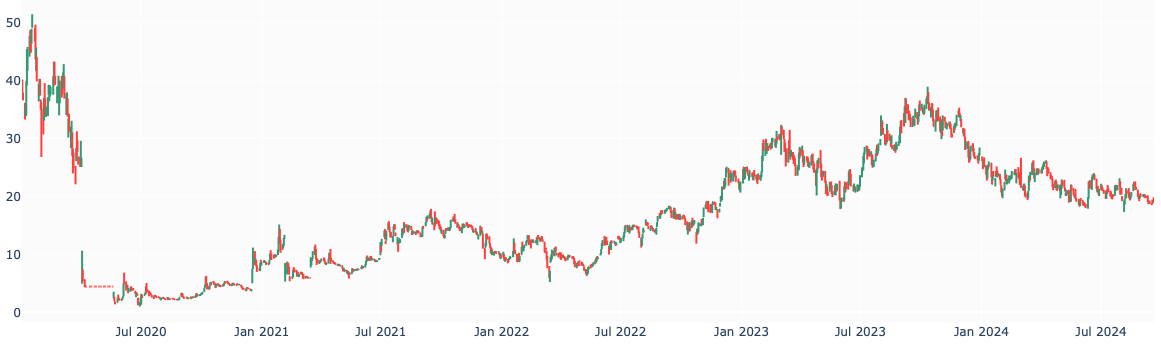
\includegraphics[width=0.8\textwidth]{pic/trend_K.jpg}
    \caption{Trend of the stock price of LuckIn Coffee.}
    \label{fig:trend_K}
\end{figure}

\begin{figure}[h]
    \centering
    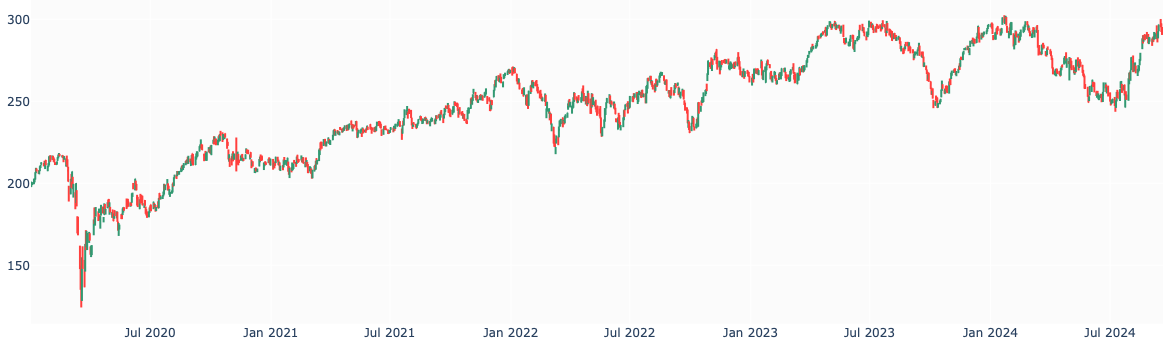
\includegraphics[width=0.8\textwidth]{pic/trend_MDC.jpg}
    \caption{Trend of the stock price of McDonald.}
    \label{fig:trend_MCD}
\end{figure}

For the XGBoost and ENet model, the accuracies are given in table \ref{tab:xgb} and table \ref{tab:enet}, respectively.
And in Fig. \ref{fig:predK} and Fig. {fig:predMDC} we show the prediction. The blue lines are the 
true stock prices. And the red line represent the predicted ones. From the results, we see the accuracies are good. 


\begin{table}[htp]
    \centering
    \caption{The prediction accuracies for stocks by XGBoost.}
    \begin{tabular}{|c|c|c|c|}
        \hline
                & MSE & MAPE & r2 \\ \hline
          LuckIn  &  5.8288   &   19.1046   & 0.4585   \\ \hline
        McDonald    &  19.0541 &     5.6457   &  0.7809 \\ \hline 
    \end{tabular}
    \label{tab:xgb}
\end{table}


\begin{table}[htp]
    \centering
    \caption{The prediction accuracies for stocks by Elastic Net Regularization.}
    \begin{tabular}{|c|c|c|c|}
        \hline
                & MSE & MAPE & r2 \\ \hline
               LuckIn  &  5.4536   &  17.3729   &  0.8361    \\ \hline
        McDonald    & 19.7565   &  5.8308   &  0.7522   \\ \hline
    \end{tabular}
    \label{tab:enet}
\end{table}


\begin{figure}[h]
    \centering
    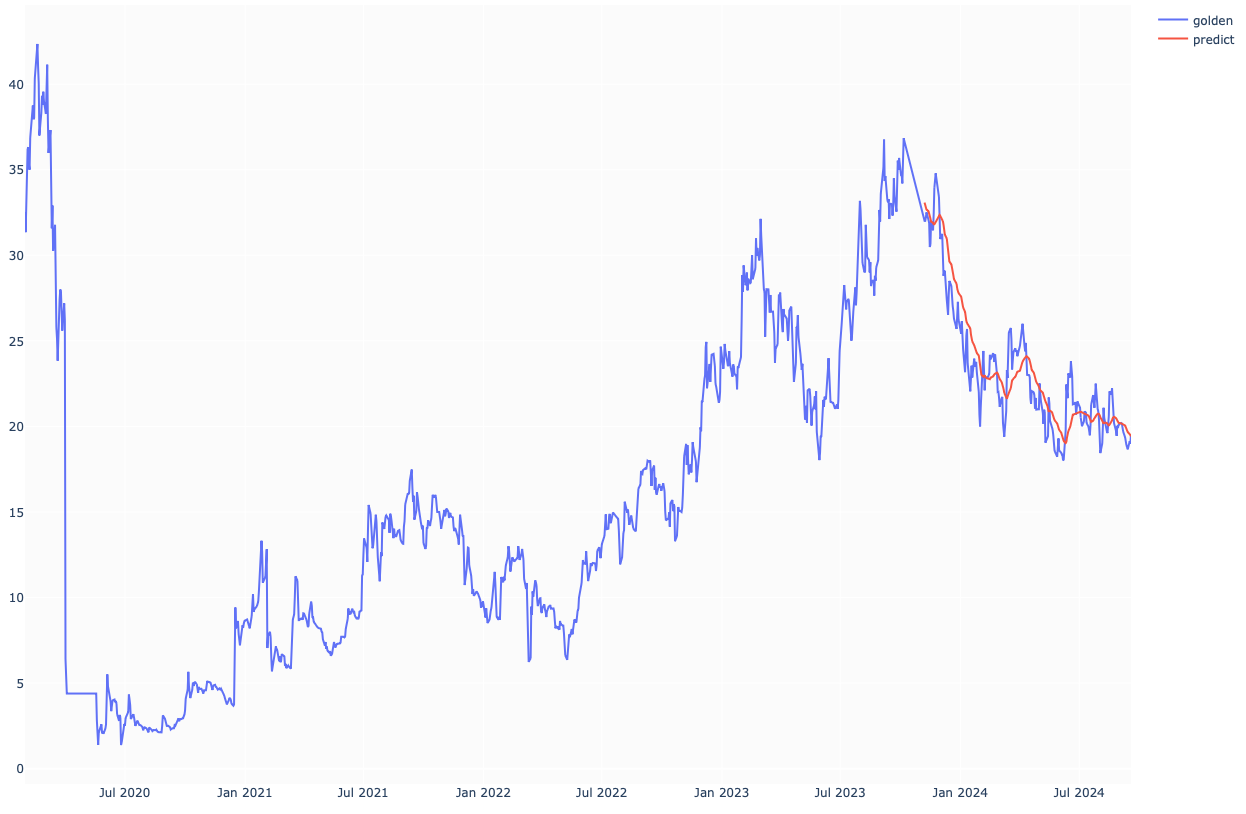
\includegraphics[width=0.8\textwidth, height=6cm]{pic/pred_K.jpg}
    \caption{Prediction of stock of LuckIn.}
    \label{fig:predK}
\end{figure}

\begin{figure}[h]
    \centering
    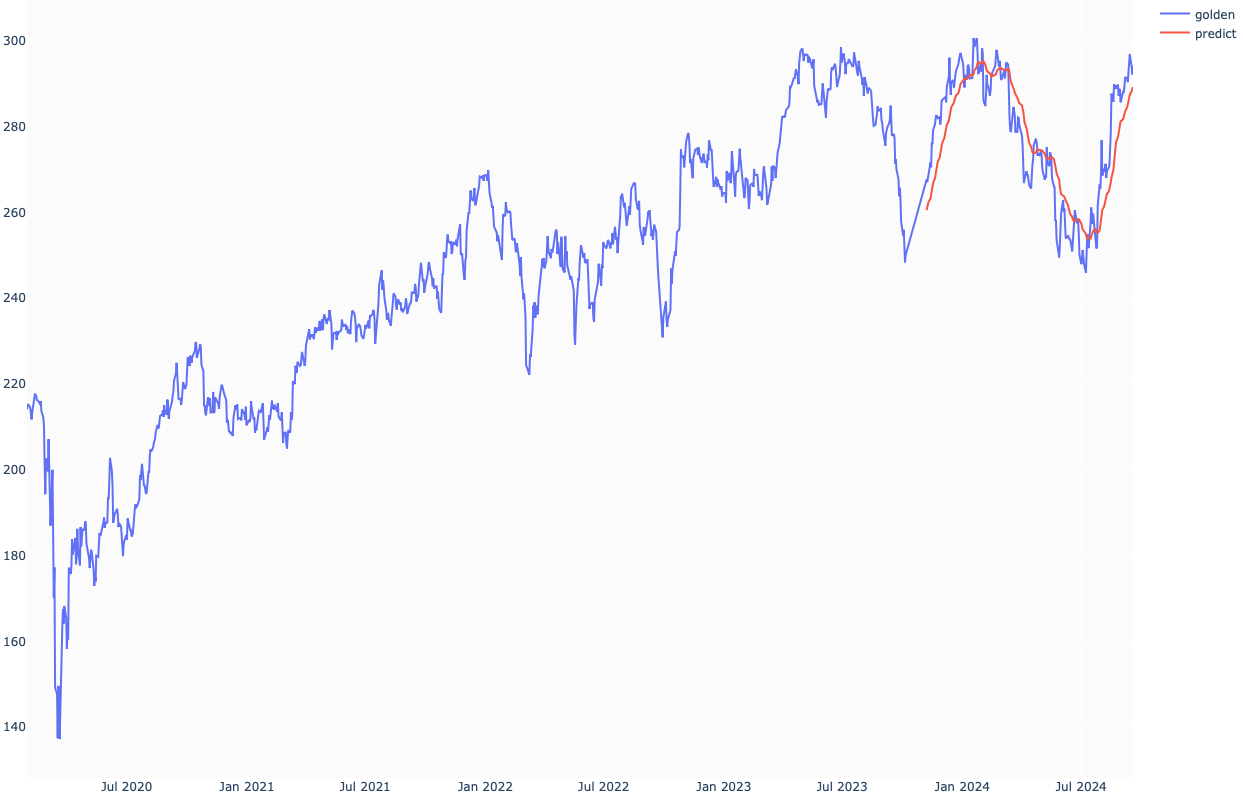
\includegraphics[width=0.8\textwidth, height=6cm]{pic/pred_MDC.jpg}
    \caption{Prediction of stock of McDonald.}
    \label{fig:predMDC}
\end{figure}


\section{Future plan}

Our next step is to explore the LSTM model. We already have the rough idea how to build it and the running time. 
We will see if we can improve our accuracy.


\section{References}

[1]� Zhuangwei Shi, Yang Hu, Guangliang Mo, Jian Wu (2021) \textbf{Attention-based CNN-LSTM and XGBoost hybrid model for stock prediction }\vspace{0.2cm}

[2] Burak G�lmez(2023) \textbf{Stock price prediction with optimized deep LSTM network with artificial rabbits optimization algorithm}\vspace{0.2cm}

[3] Tran Phuoc, Pham Thi Kim Anh, Phan Huy Tam,  \& Chien V. Nguyen (2024)\textbf{Applying machine learning algorithms to predict the stock price trend in the stock market in Vietnam}\vspace{0.2cm}



\end{document}
